Results presented here were obtained from the data collected by the \STAR\ experiment at \RHIC\ in the year 2011 for \AuAu\ collisions at \sNN\ = 200 GeV. The data set was taken using minimum bias trigger. A total $\sim$113.9 good events out of total 121 events.

\FloatBarrier
\subsection{Event selection}

Analyzed events were required to have a primary vertex position along the longitudinal direction ($V_z$) within 30~cm from the center of the Time Projection Chamber (\TPC). In addition, $V_r\equiv\sqrt{V_x^2+V_y^2}<2$~cm cut was implemented to minimize interactions between beam and beam pipe as well as $|V_z - Vpd_z| < 3$~cm cut to suppress pile-up effects. The distributions of the Z-component of the vertex and $V_z-Vpd_z$ are shown on the \cref{fig:VtxZCuts}. X and Y projections of the vertex before and after event selection are shown on the \cref{fig:VtxXYCuts}.
The event selection cuts are displayed in the \cref{tab:EventCuts}.

\begin{table}[th]
    \centering
    \begin{tabular}{|c|c|c|c|}
         \hline
        Data & Vertex$_z$ & Vertex$_r$ & Vertex$_z - $Vpd$_z$ \\
         \hline
        \AuAu\ 200 GeV & $|V_z|<30$ cm & $|V_r|<2$ cm & $|V_z - Vpd_z|<3$ cm \\
         \hline
    \end{tabular}
    \caption{Event selection cuts.}
    \label{tab:EventCuts}
\end{table}

\begin{figure}[ht]
    \begin{subfigure}{.49\textwidth}
        \centering
        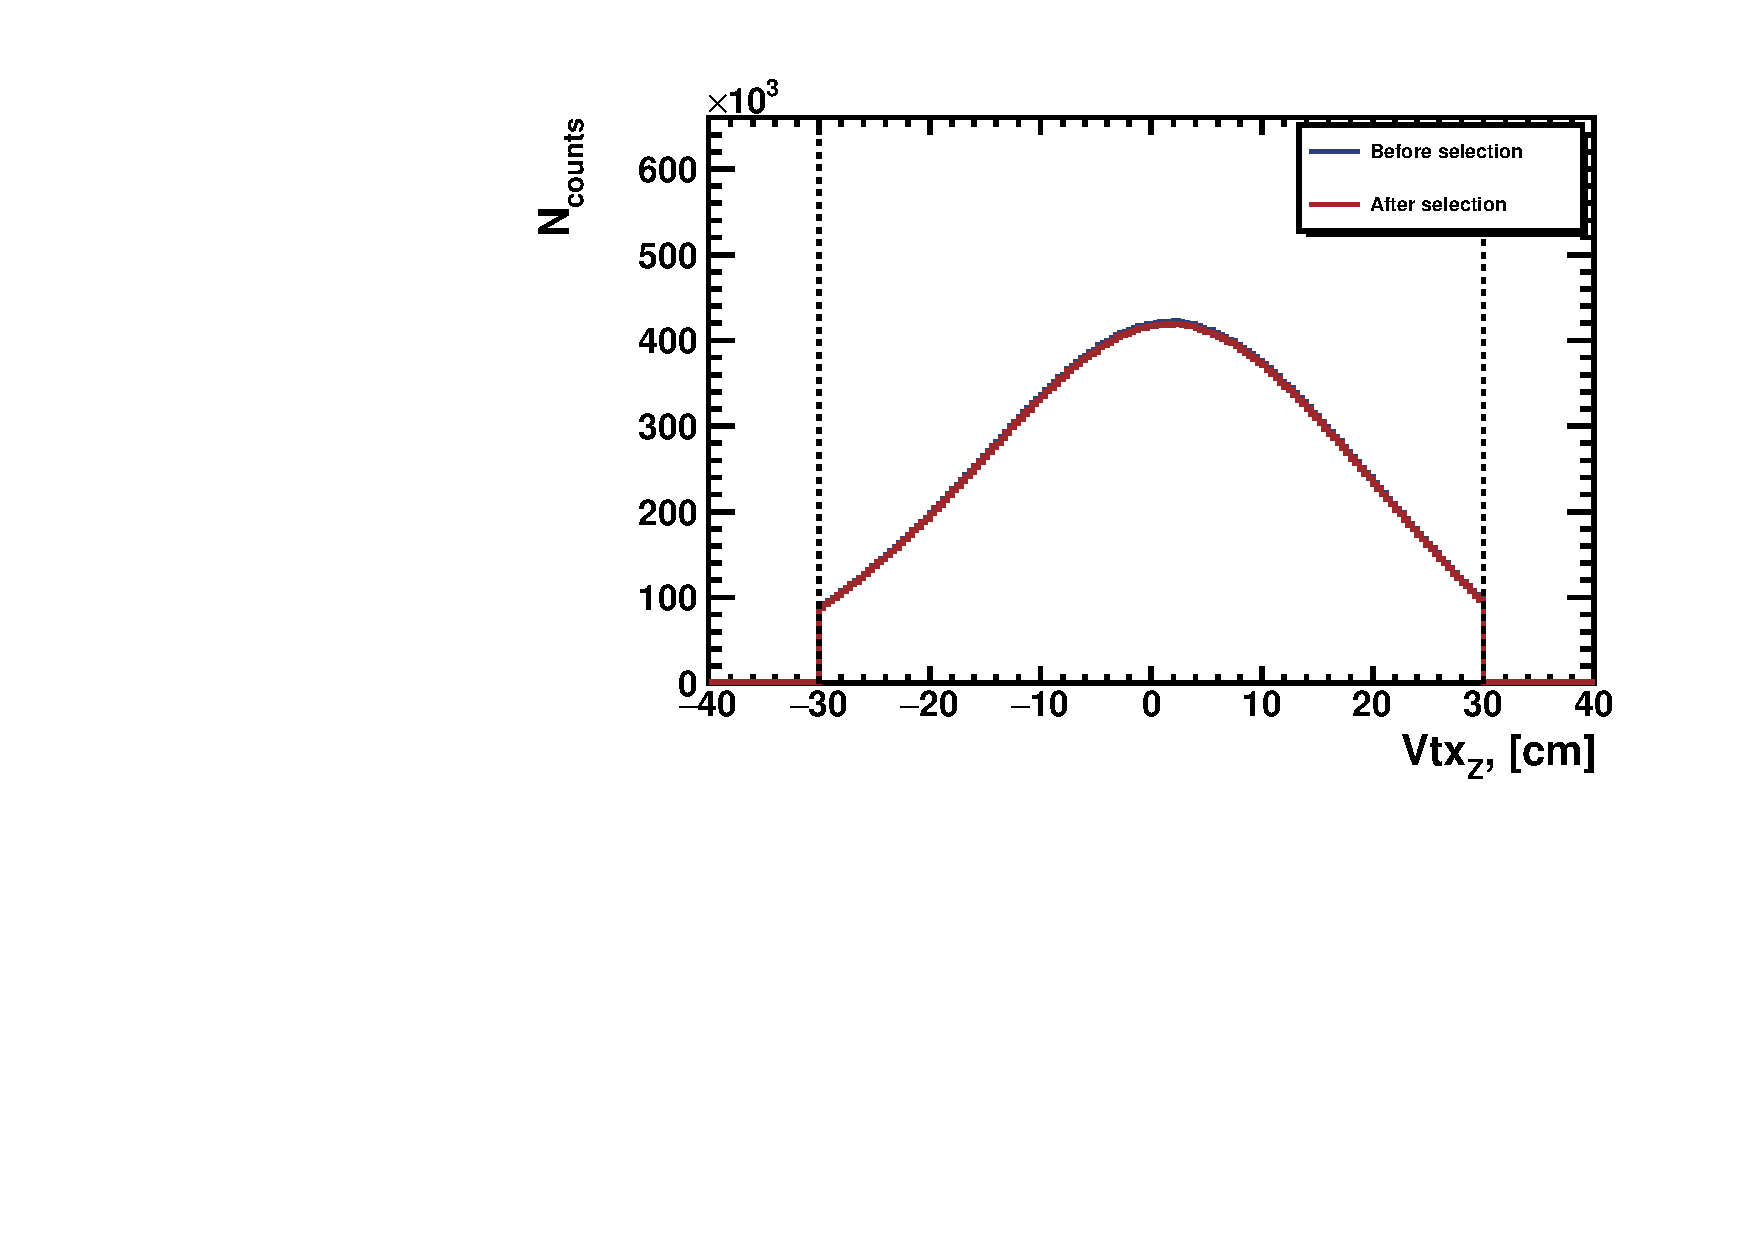
\includegraphics[width=1.\linewidth]{Figures/VtxZ.pdf}
        %\caption{a}
    \end{subfigure}
    \begin{subfigure}{.49\textwidth}
        \centering
        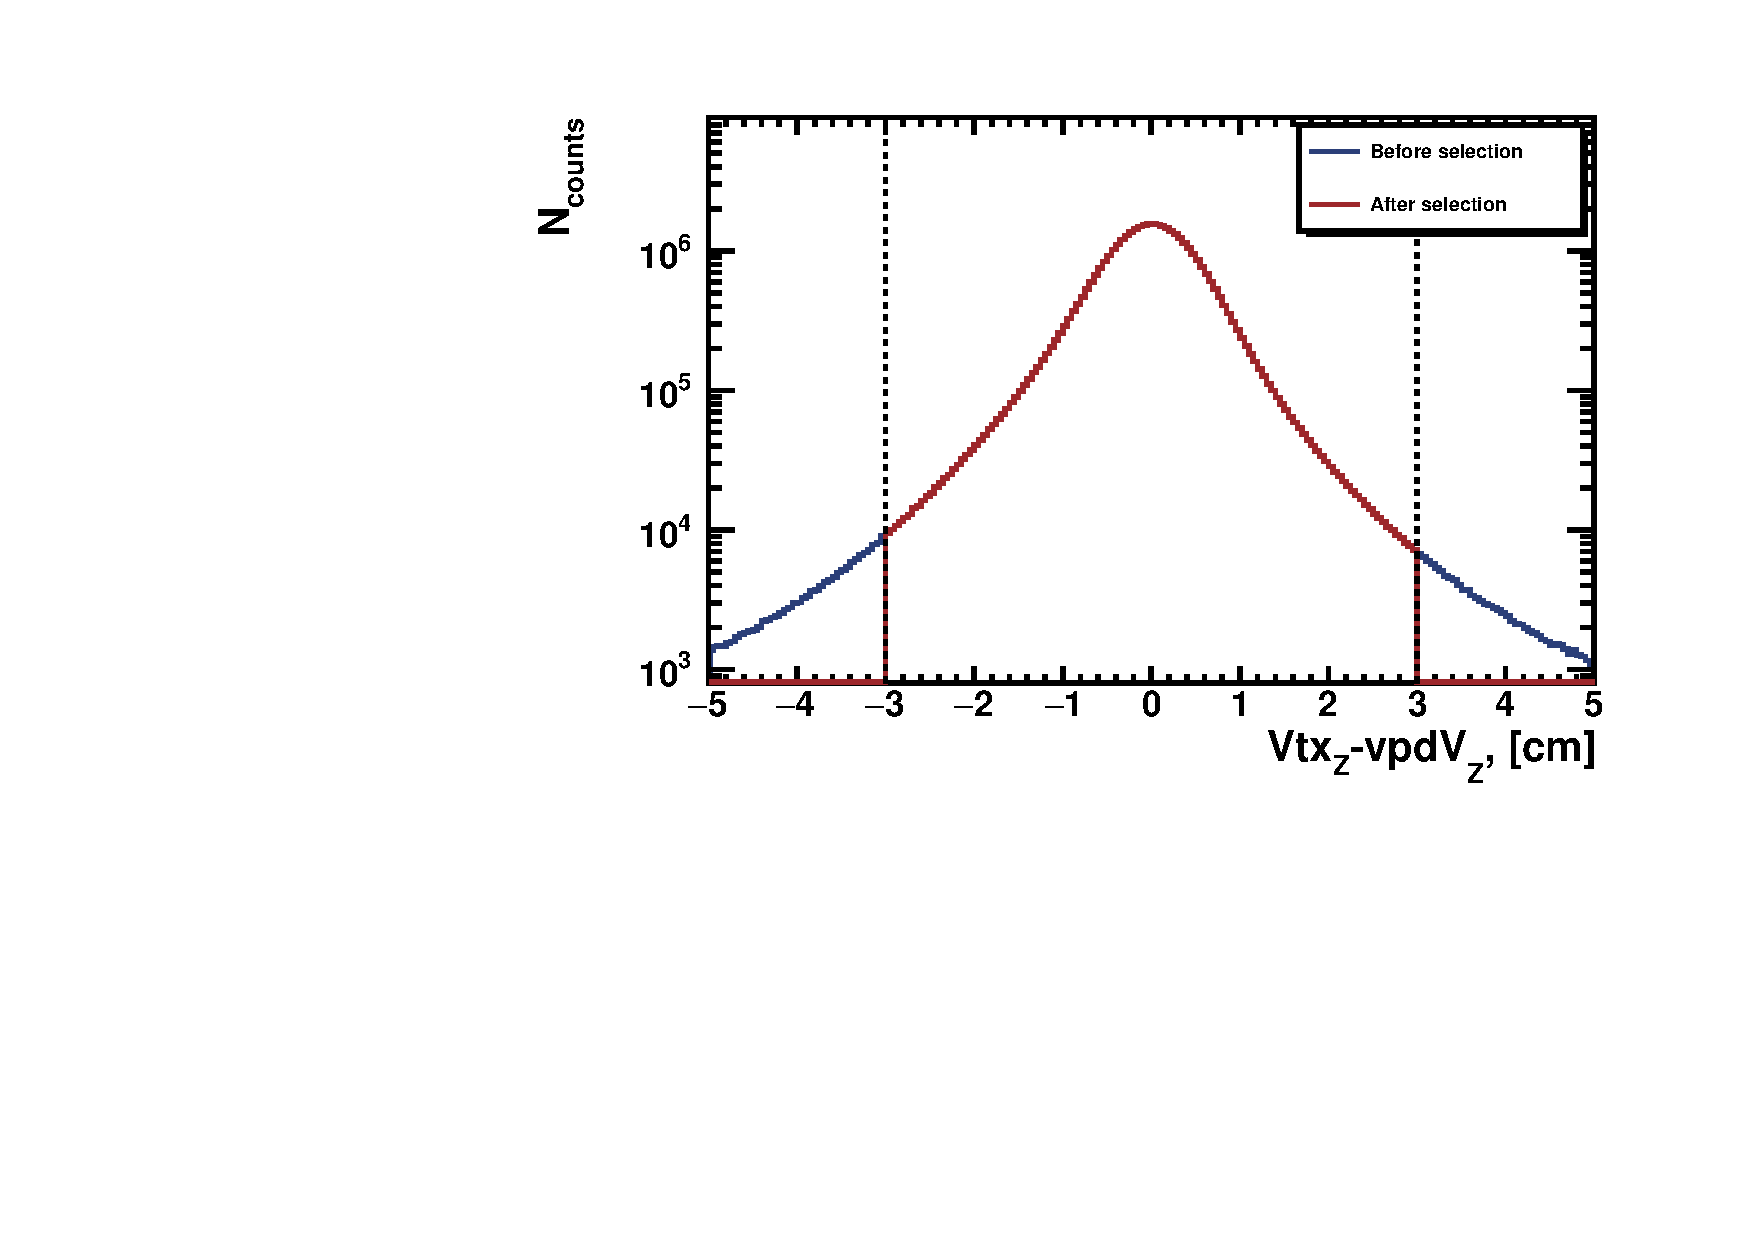
\includegraphics[width=1.\linewidth]{Figures/VtxVpdZ.pdf}
        %\caption{b}
    \end{subfigure}
    \caption{Distribution of the $Vtx_Z$ (left) and $Vtx_Z - Vpd_Z$ (right).}
    \label{fig:VtxZCuts}
\end{figure}

\begin{figure}[ht]
    \begin{subfigure}{.49\textwidth}
        \centering
        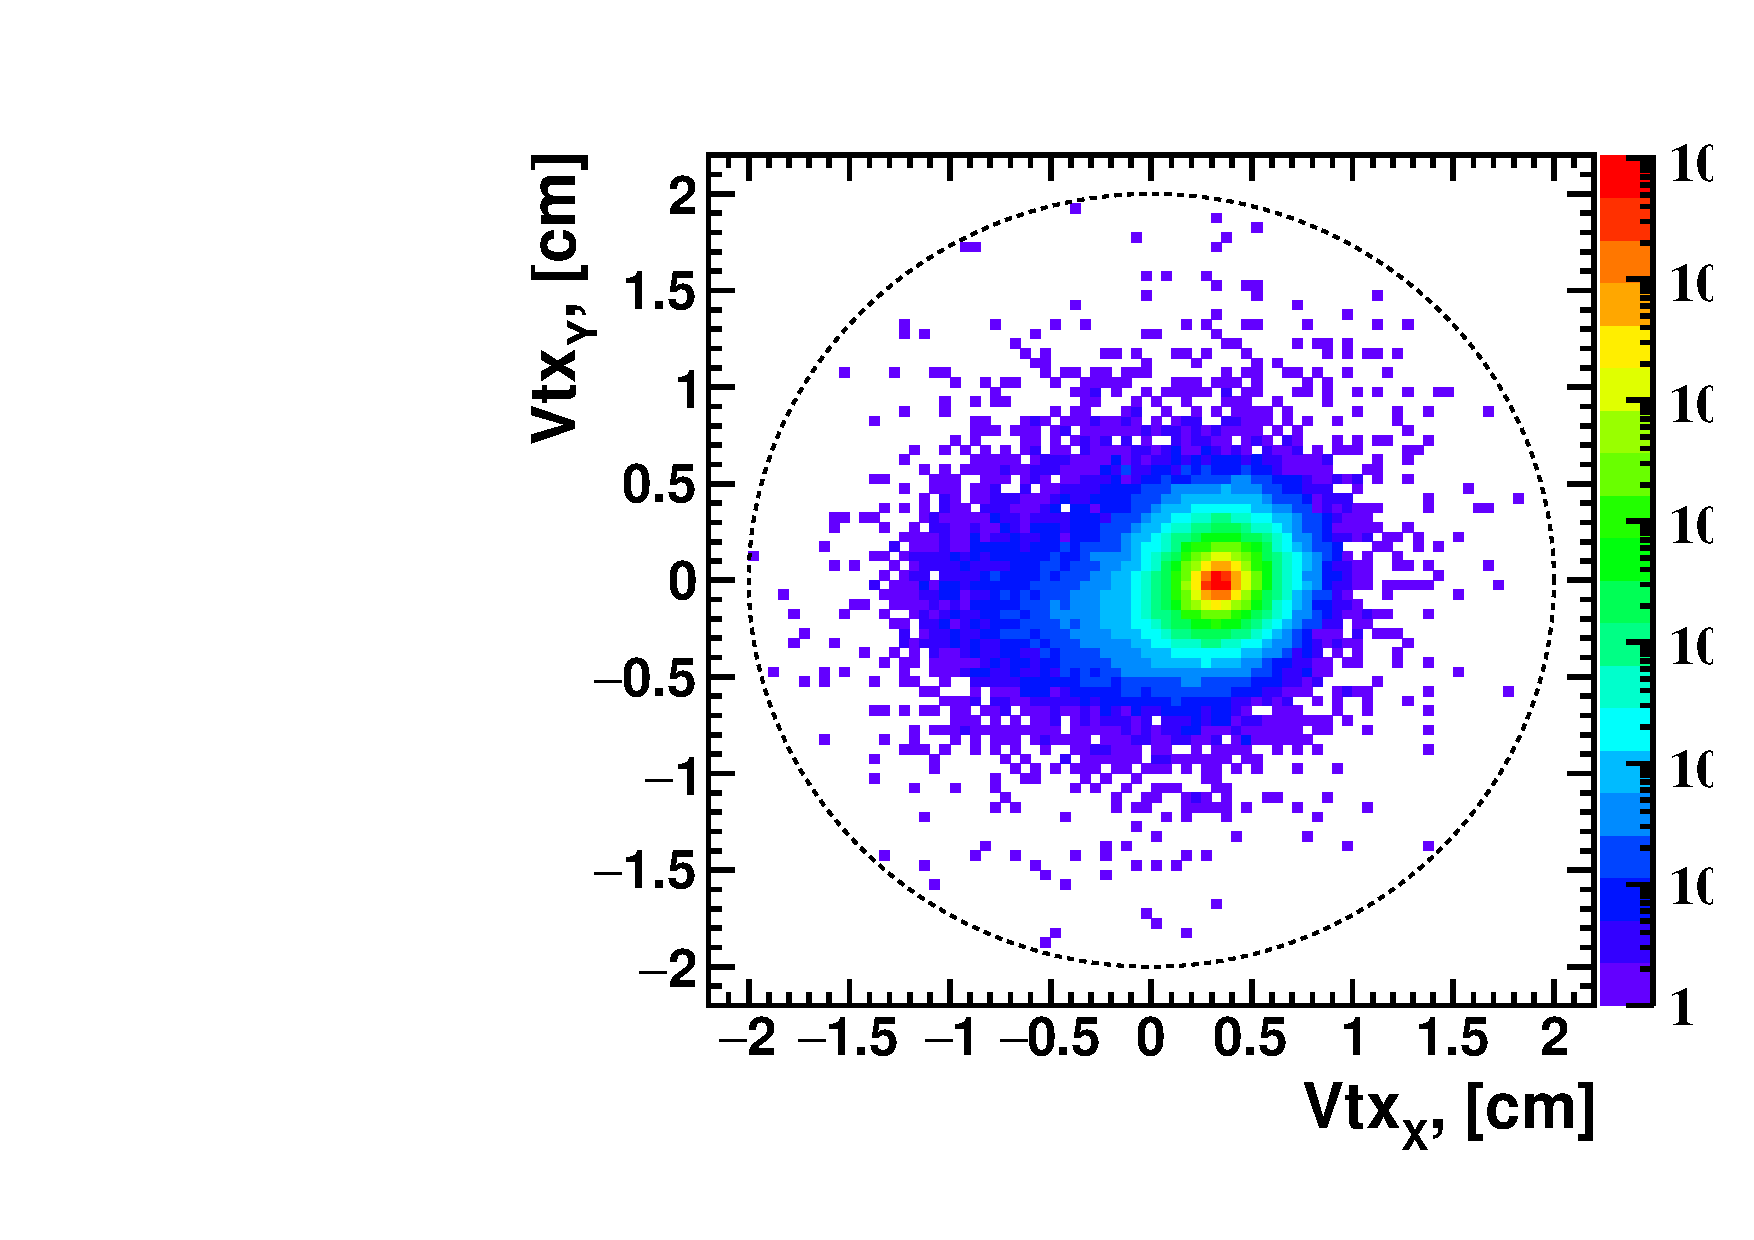
\includegraphics[width=1.\linewidth]{Figures/VtxXY0.pdf}
        %\caption{a}
    \end{subfigure}
    \begin{subfigure}{.49\textwidth}
        \centering
        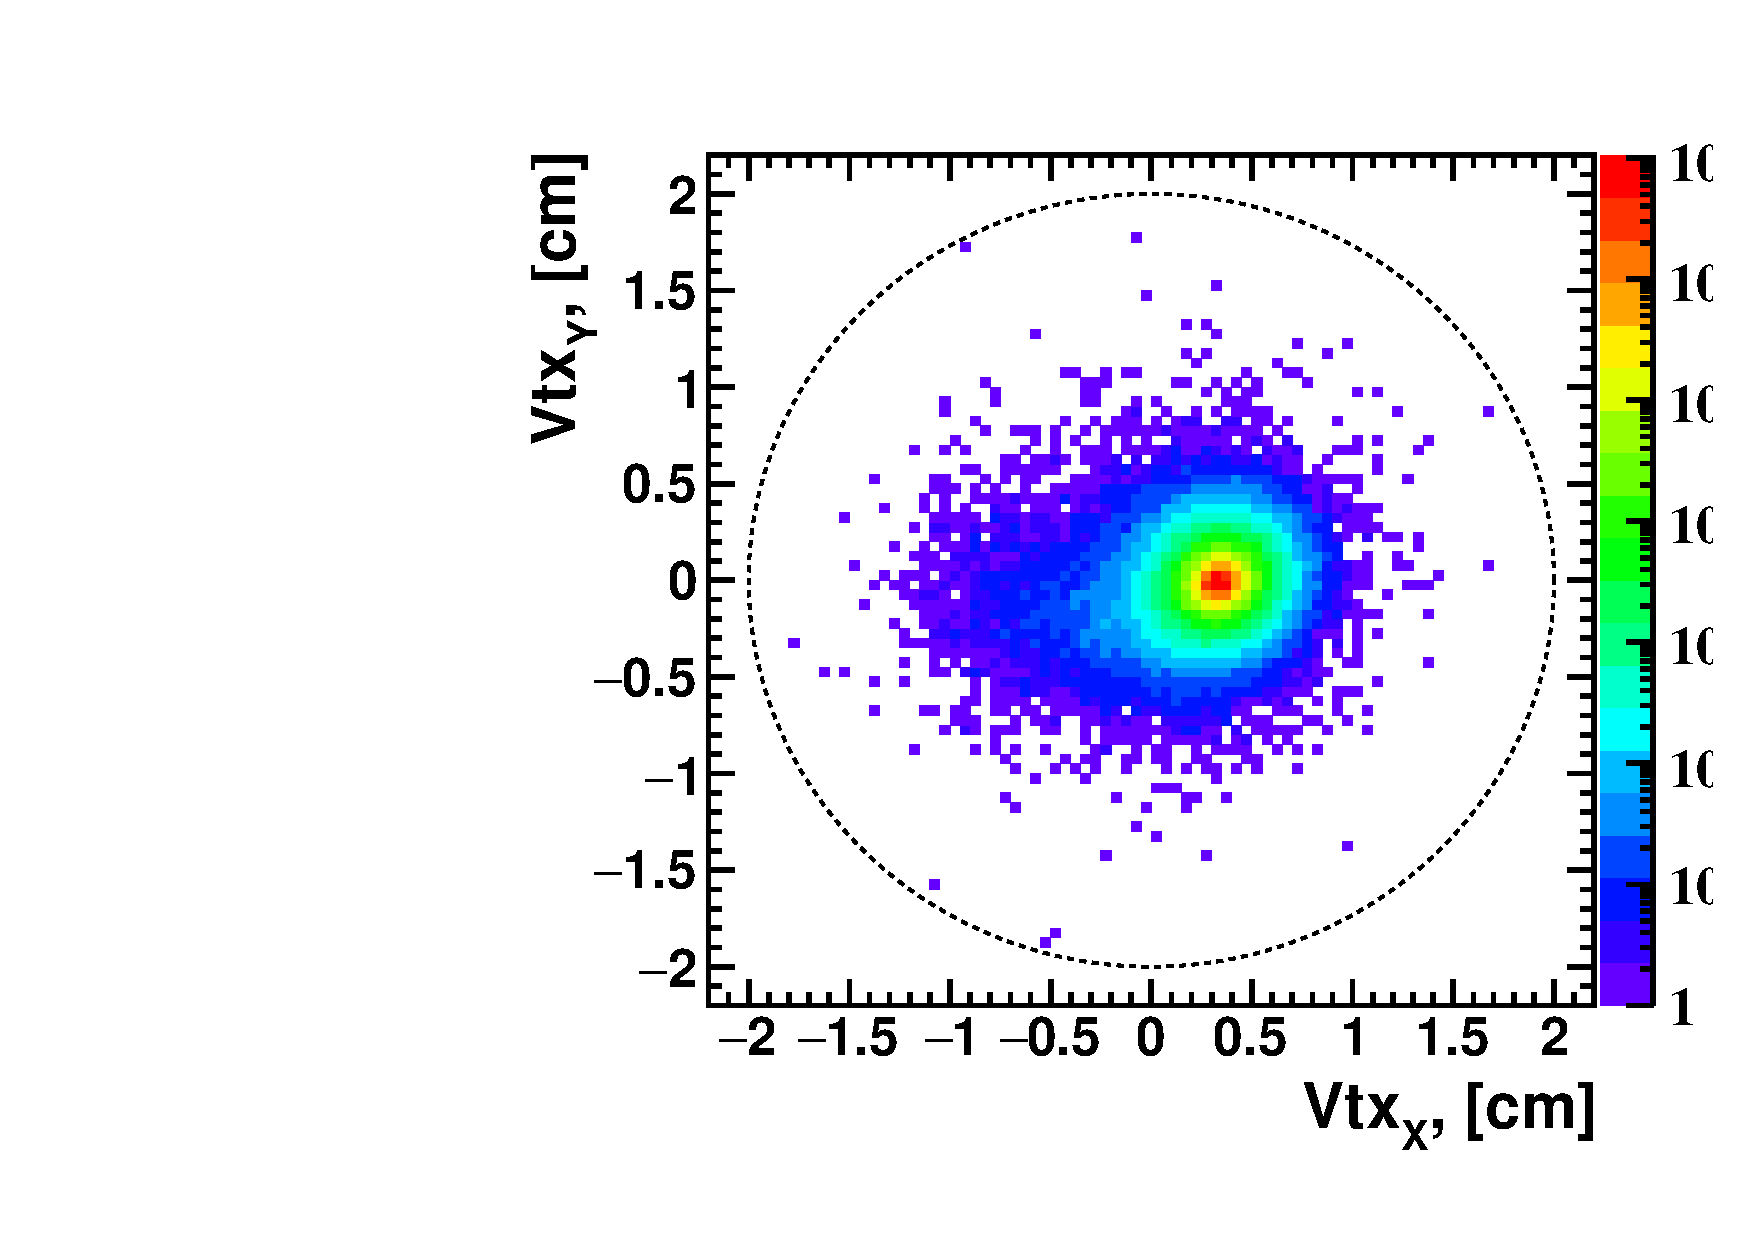
\includegraphics[width=1.\linewidth]{Figures/VtxXY1.pdf}
        %\caption{b}
    \end{subfigure}
    \caption{Distribution of the X- and Y-components of the vertex before (left) and after (right) event selection.}
    \label{fig:VtxXYCuts}
\end{figure}

\FloatBarrier
\subsection {Track selection}

Only primary tracks were used in the analysis. Cuts for number of fit points $N_{hits}$ and its ratio to the number of total possible hit points $N_{hits}^{Poss}$ were implemented to ensure accurate reconstructed track momentum and to minimize the effect of track-splitting. The additional distance of closest approach (\DCA) cut was used to suppress the tracks from secondary vertices. All cuts for track selection are shown in the \cref{tab:TrackCuts}.

\begin{table}[th]
    \centering
    \begin{tabular}{|c|c|}
        \hline
        \textbf{Track parameter} & \textbf{Cut} \\
        \hline
        Transverse momentum & $p_{T}>0.15$ GeV/c \\
        \hline
        Distance of closest approach & $|$\DCA$|<3$ cm \\
        \hline
        Number of fit points & $N_{hits}>15$ \\
        \hline
        No. of fit points to No. of possible points ratio & $N_{hits}/N_{hits}^{Poss} \geqslant 0.51$ \\
        \hline
        Pseudorapidity & $|\eta|<1$ \\
        \hline
        Total momentum & $p<10$ GeV/c \\
        \hline
    \end{tabular}
    \caption{Track selection cuts.}
    \label{tab:TrackCuts}
\end{table}

\begin{figure}[ht]
    \begin{subfigure}{.49\textwidth}
        \centering
        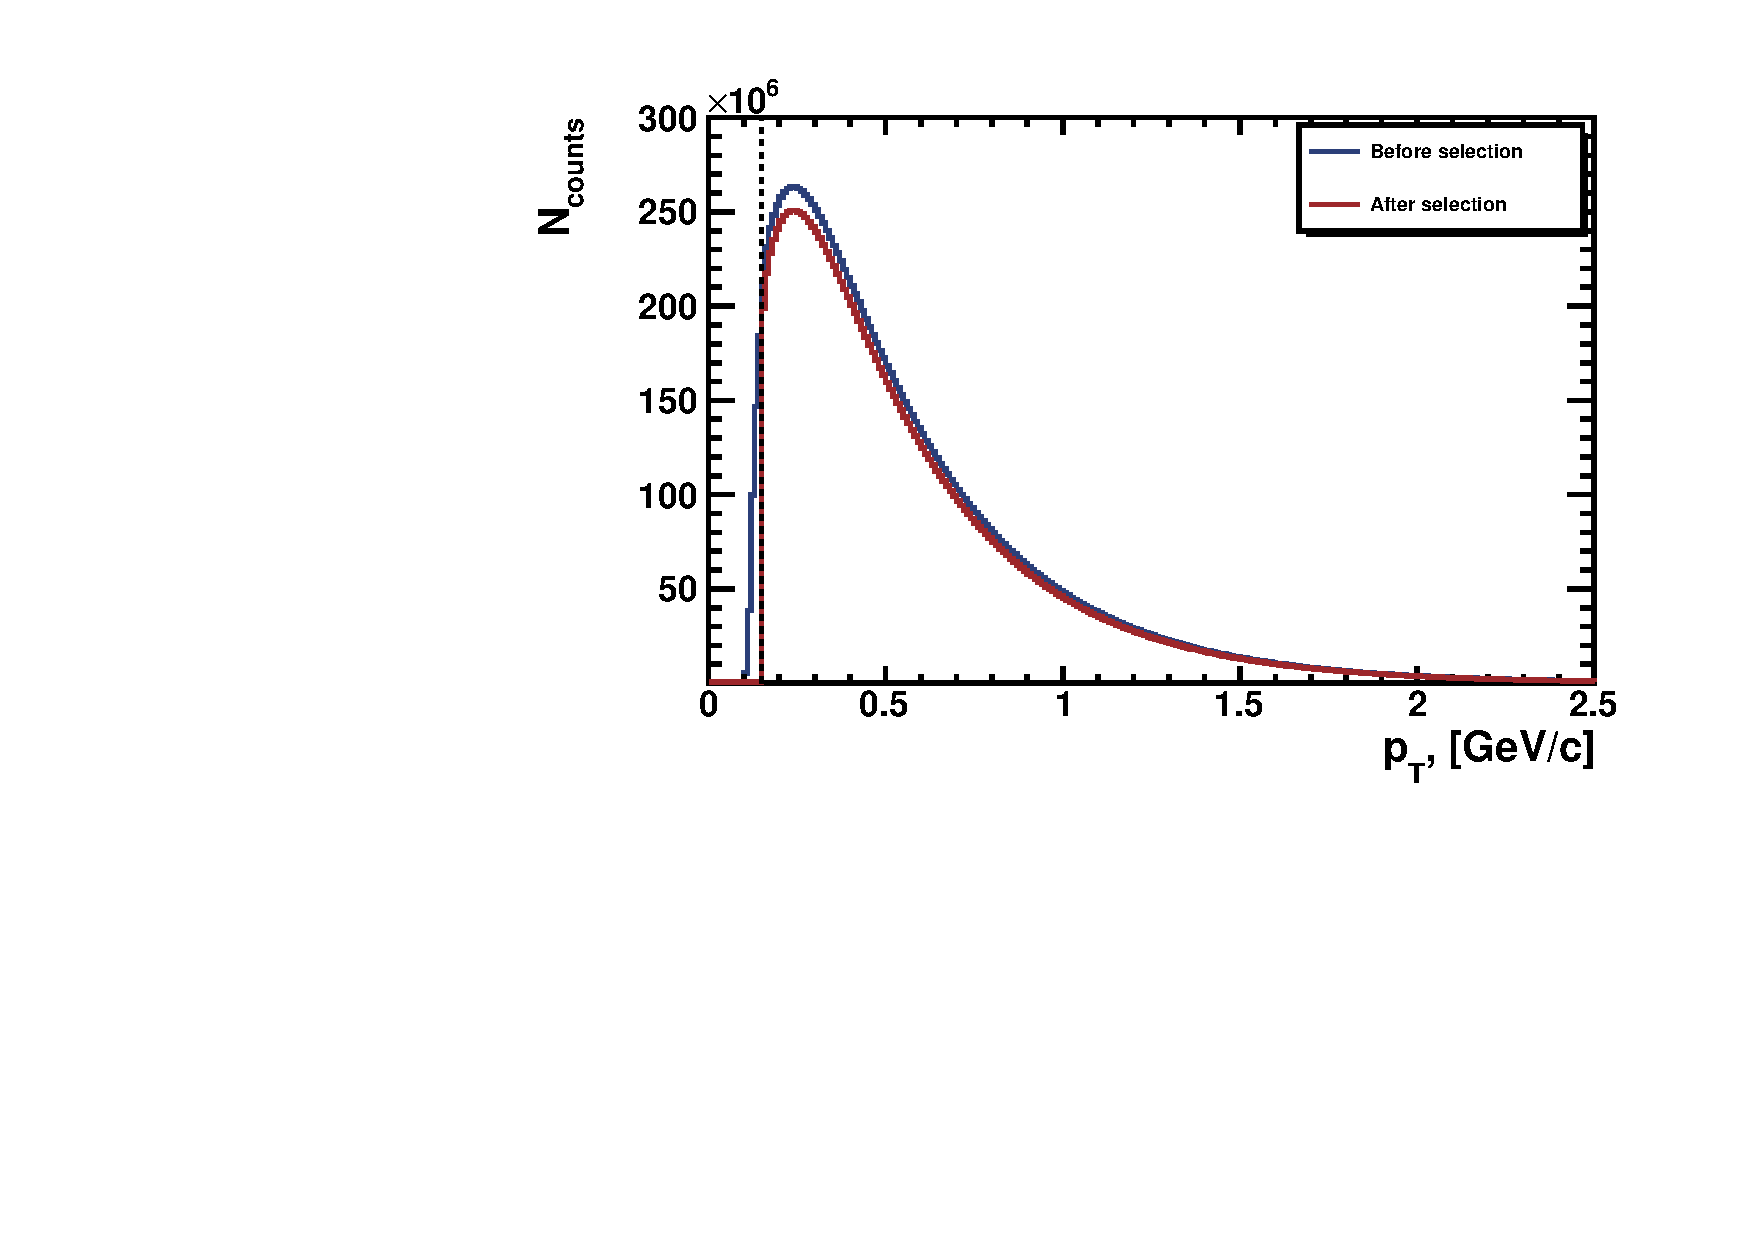
\includegraphics[width=1.\linewidth]{Figures/Pt.pdf}
        %\caption{a}
    \end{subfigure}
    \begin{subfigure}{.49\textwidth}
        \centering
        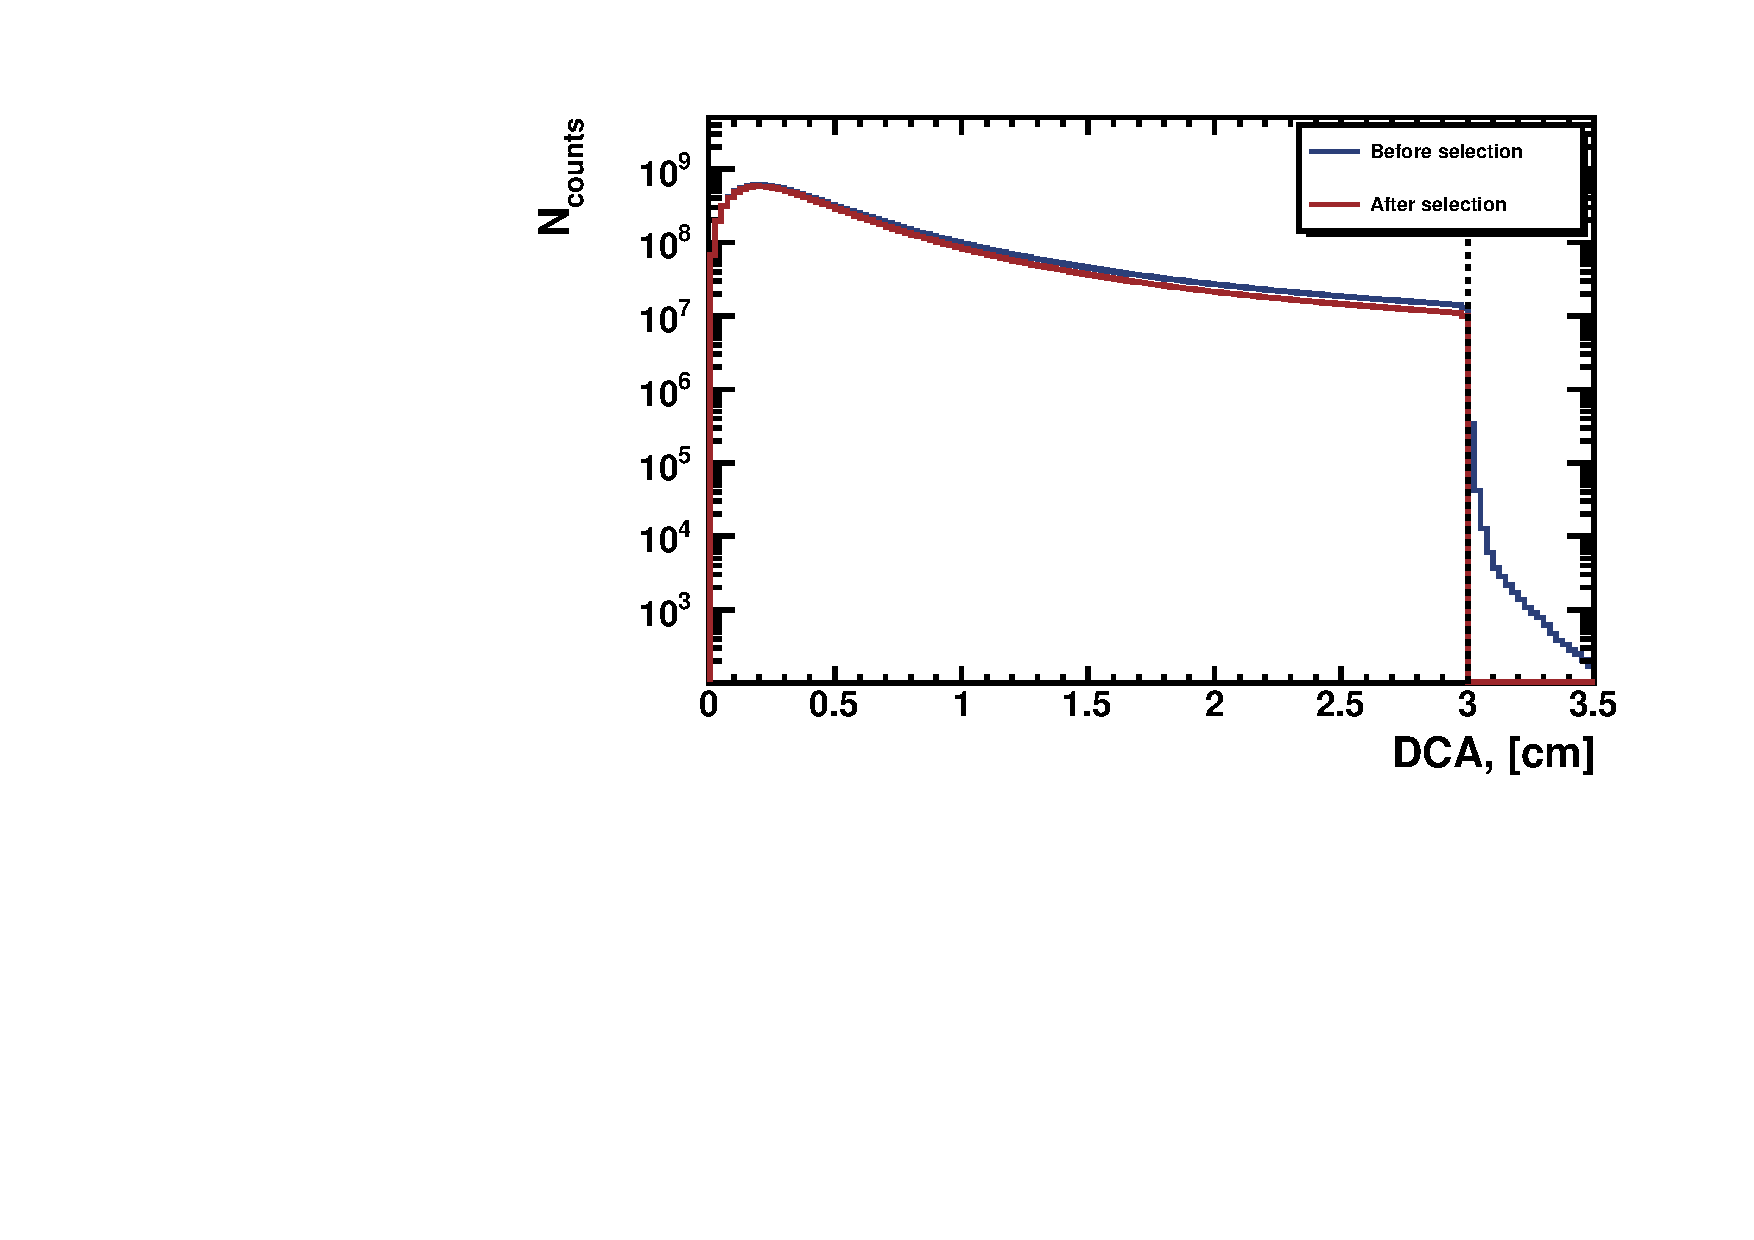
\includegraphics[width=1.\linewidth]{Figures/DCA.pdf}
        %\caption{b}
    \end{subfigure}
    \\
    \begin{subfigure}{.49\textwidth}
        \centering
        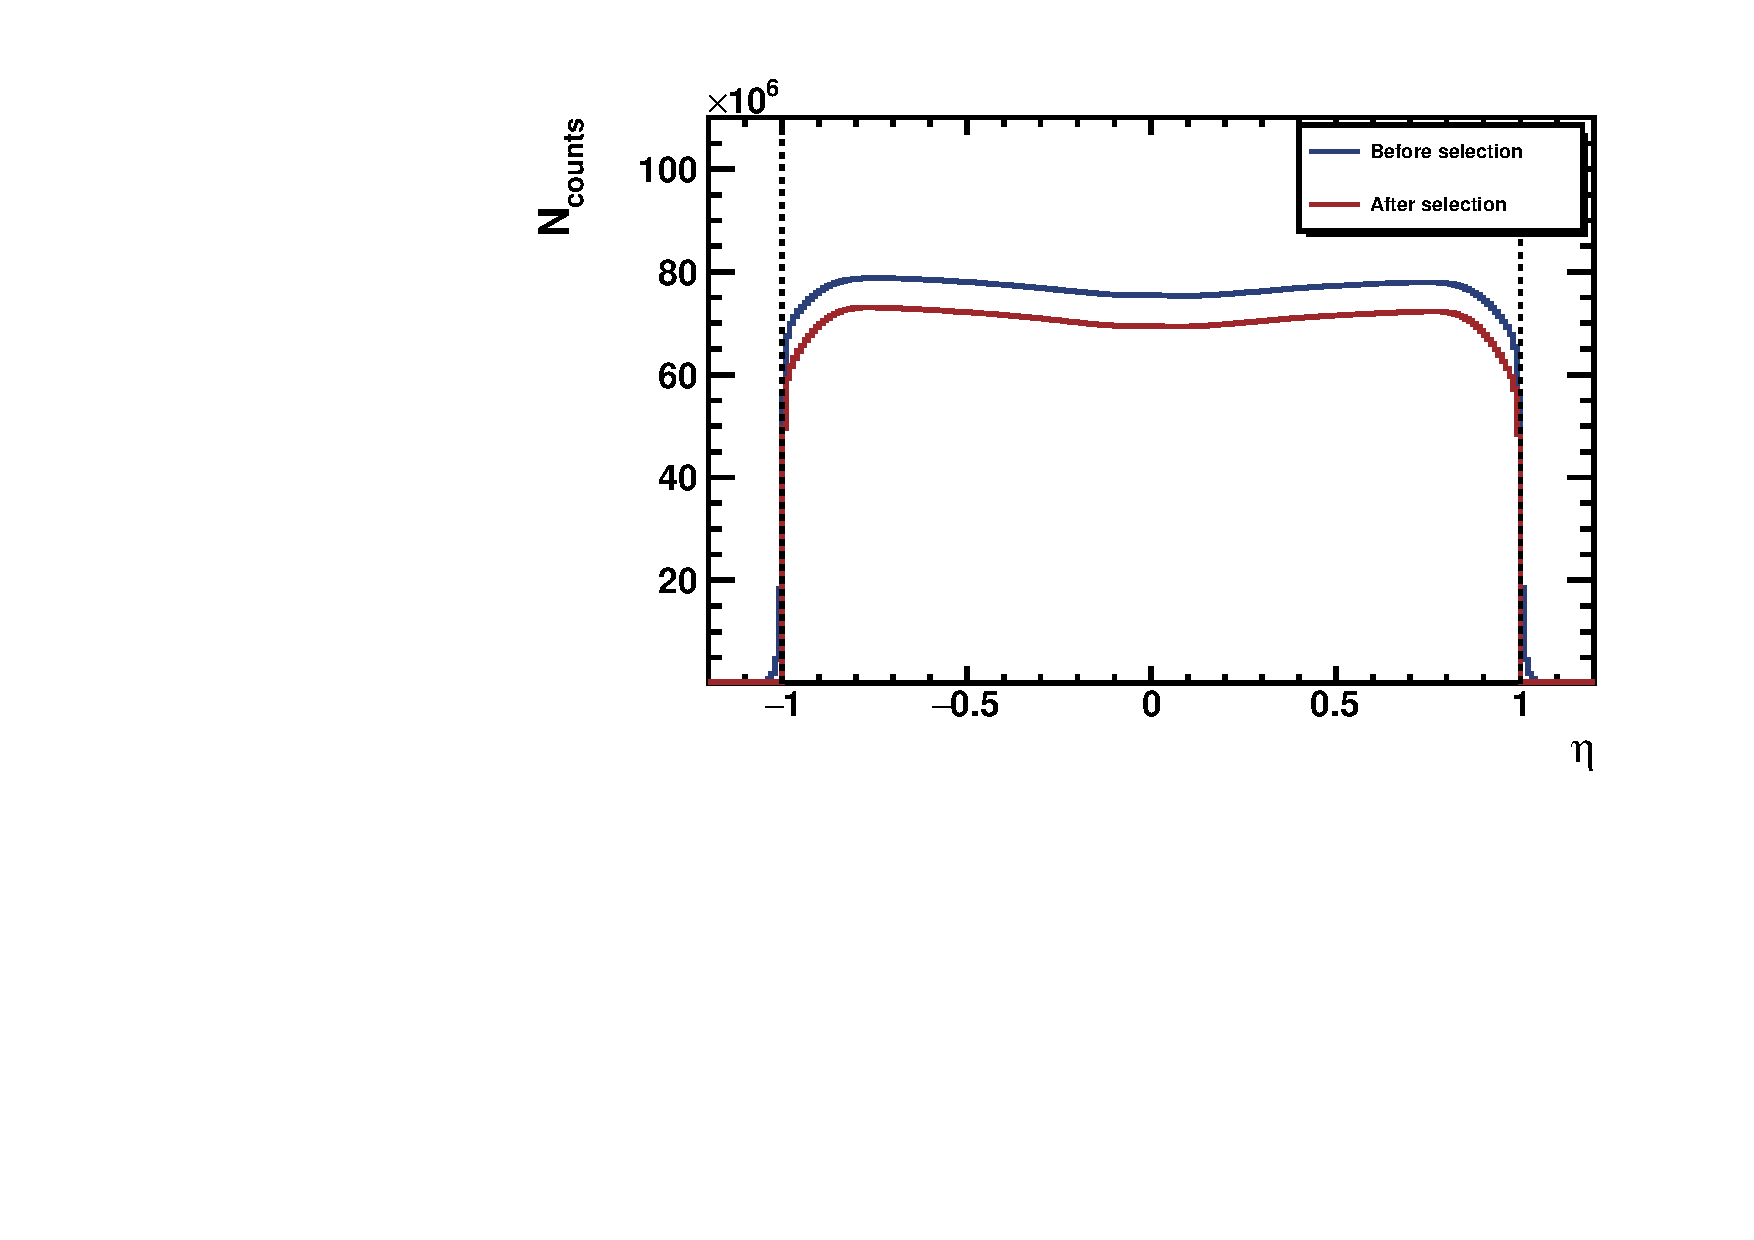
\includegraphics[width=1.\linewidth]{Figures/Eta.pdf}
        %\caption{a}
    \end{subfigure}
    \begin{subfigure}{.49\textwidth}
        \centering
        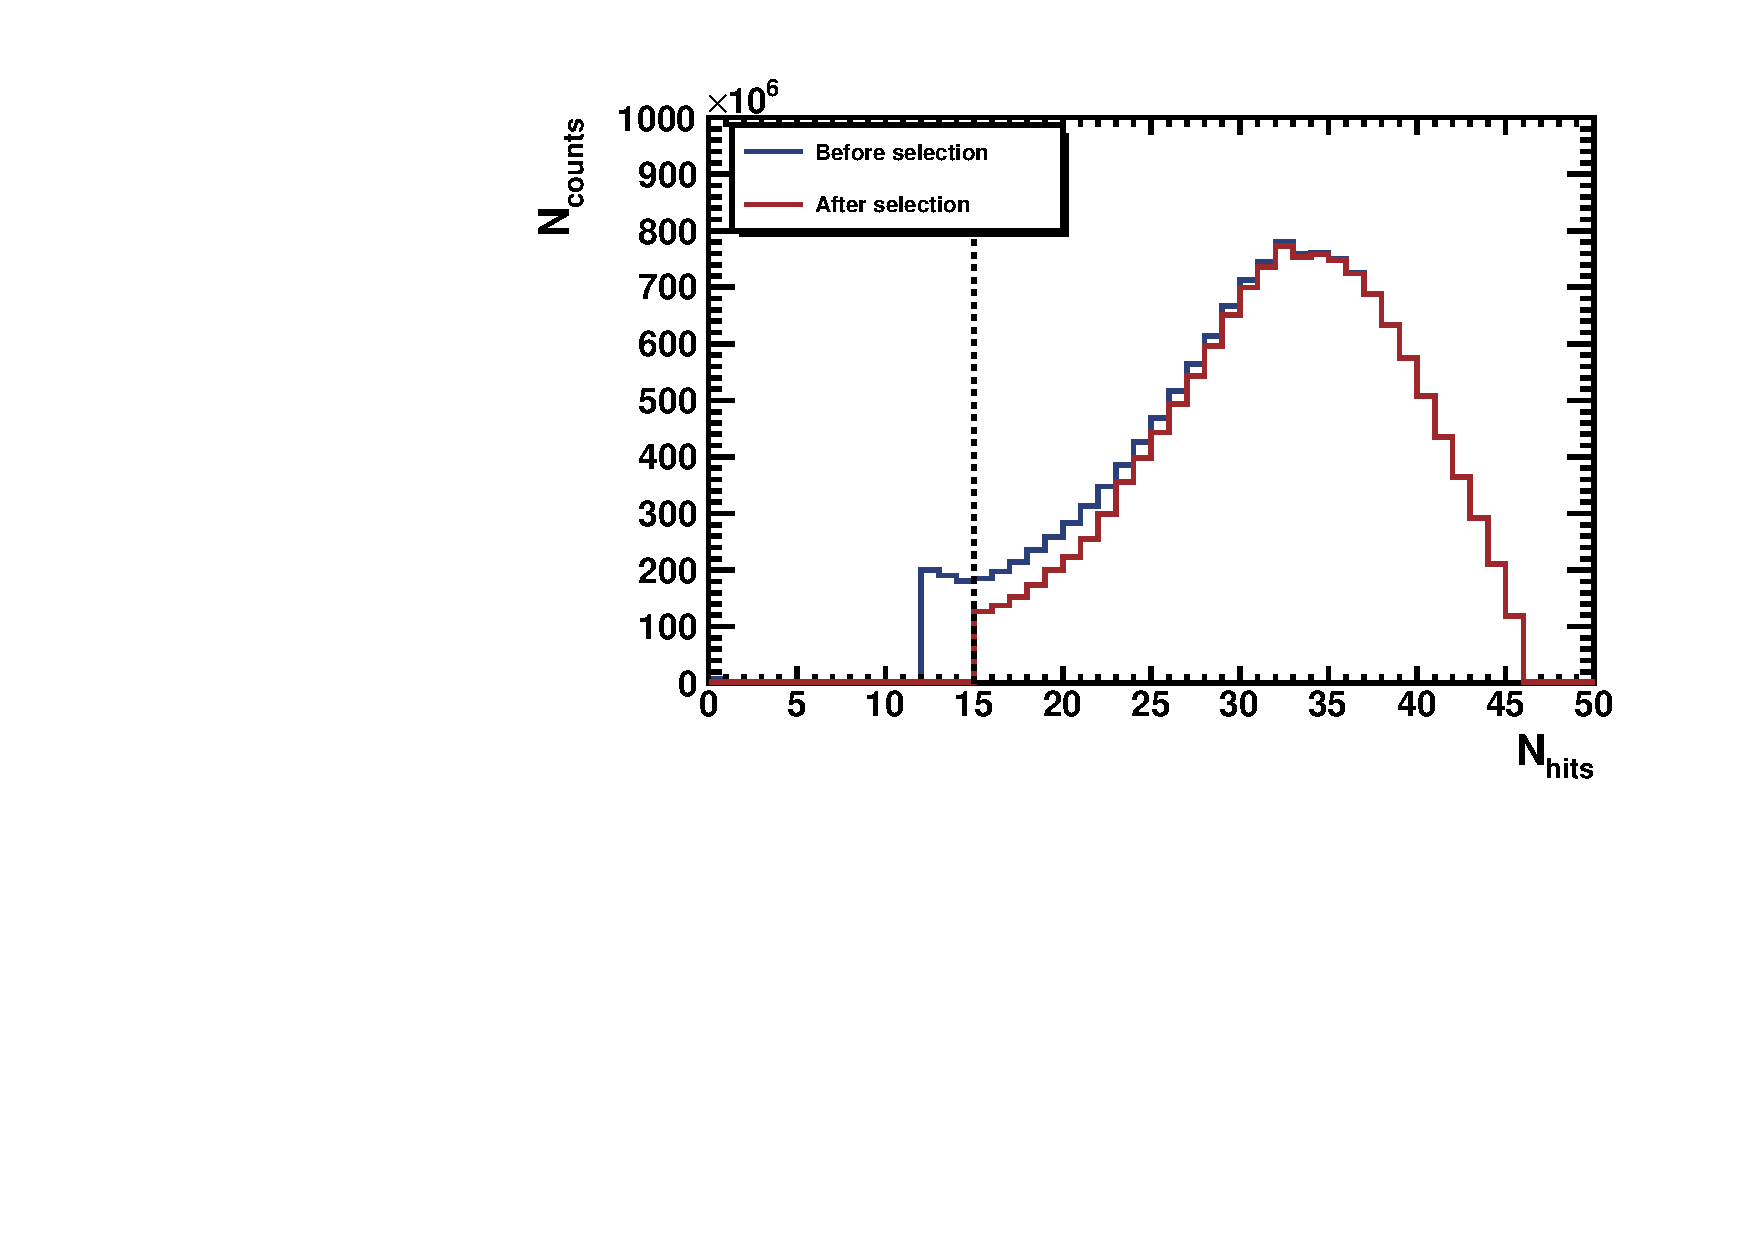
\includegraphics[width=1.\linewidth]{Figures/Nhits.pdf}
        %\caption{b}
    \end{subfigure}
    \caption{(upper left) $p_T$-distribution, (upper right) $|$\DCA$|$, (bottom left) $\eta$ and (bottom right) $N_{hits}$ distributions before and after track selection.}
    \label{fig:TrackSelection}
\end{figure}

\FloatBarrier
\subsection {Particle identification}

\begin{figure}[ht]
    \begin{subfigure}{.49\textwidth}
        \centering
        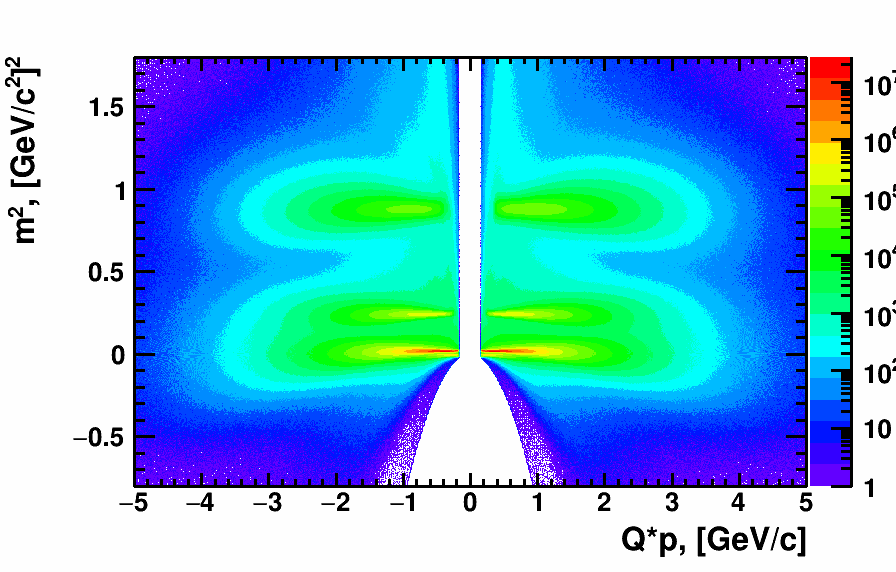
\includegraphics[width=1.\linewidth]{Figures/M2Qp_before_PID.png}
        %\caption{a}
    \end{subfigure}
    \begin{subfigure}{.49\textwidth}
        \centering
        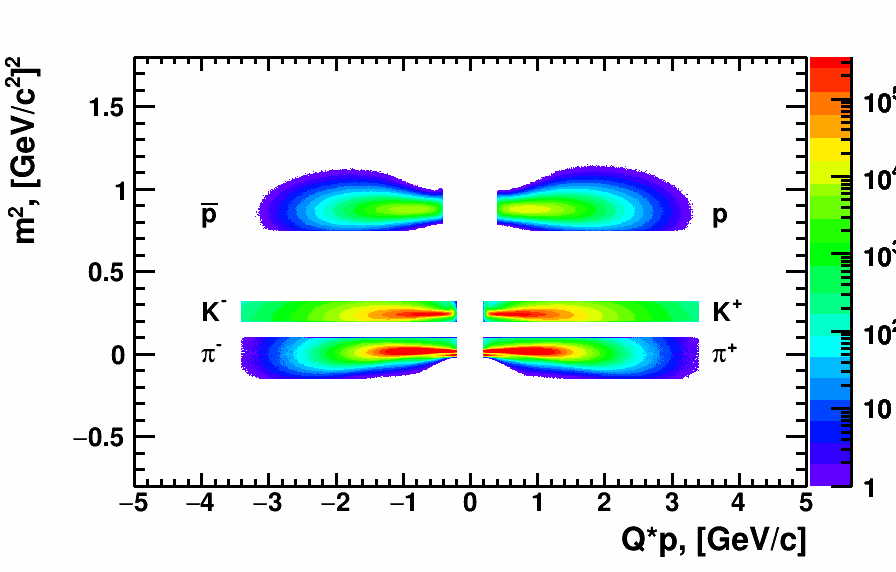
\includegraphics[width=1.\linewidth]{Figures/M2Qp_after_PID.png}
        %\caption{b}
    \end{subfigure}
    \label{fig:M2vsQp}
    \caption{$m^2$ estimated using \TPC\ and \TOF\ detectors vs charged total momentum $Q\cdot p$ before (left) and after (right) \PID\ procedure.}
\end{figure}